
\documentclass[10pt]{article}
\usepackage[margin=0.7in]{geometry}
\usepackage{graphicx}
\usepackage{booktabs}
\usepackage{longtable}
\usepackage{array}
\usepackage{hyperref}
\usepackage{xcolor}
\usepackage{float}
\usepackage{caption}
\hypersetup{colorlinks=true, linkcolor=blue, urlcolor=blue}
\setlength{\parindent}{0pt}
\setlength{\parskip}{4pt}
\renewcommand{\arraystretch}{1.12}

\title{Quantum Junction Challenge: Condensed Codex Session Report}
\author{Codex run summary}
\date{Built 2026-06-06 06:33:07 }

\begin{document}
\maketitle

\section*{Executive Summary}
The session produced selected peak bitstrings for \textbf{40/49} challenge files. The remaining blanks are
\texttt{64\_40, 104\_49, 48\_42, 56\_43, 64\_44, 72\_45, 80\_46, 88\_47, 96\_48}. The selected set contains \textbf{10} exact statevector answers and
\textbf{30} tensor-network or MPS-derived candidates. Among the approximate selected rows, \textbf{17}
are from the canonical Quimb GPU pass, \textbf{11} from canonical Quimb CPU, and \textbf{1} from an RCM-order CPU
fallback. Exact statevector peaks had mean peak probability 0.513 and mean gap to the second bitstring
0.459.

The main result is a usable candidate set, not a proof of correctness for every approximate row. Easy and moderate
instances often had large sampled peak fractions and/or corroborating evidence. Several hard rows are weak: they were
selected because they were the best available evidence, but their sampled top fractions are near one or two samples out of
512/1024. The session later pivoted away from long-running graph-MPS sweeps after the user set a practical
``about 2 hours'' per-attempt budget.

\section*{Candidate Selection Rule}
The collector selected one answer per challenge using source priority, then evidence consistency. The priority order used in
the current collector was: exact statevector, canonical Quimb GPU, optimized-U3 GPU, canonical Quimb CPU, MPO-unswap, RCM/MST/
degree/mid/fast/identity CPU fallbacks, sparse beam, and low-priority Aer MPS pilot evidence. Exact answers were accepted
directly. Approximate answers were chosen as sampled top bitstrings in Qiskit/counts order, with the right-most bit
corresponding to qubit 0. When multiple methods agreed on the same bitstring, the report records that as higher evidence
count.

\begin{figure}[H]
\centering
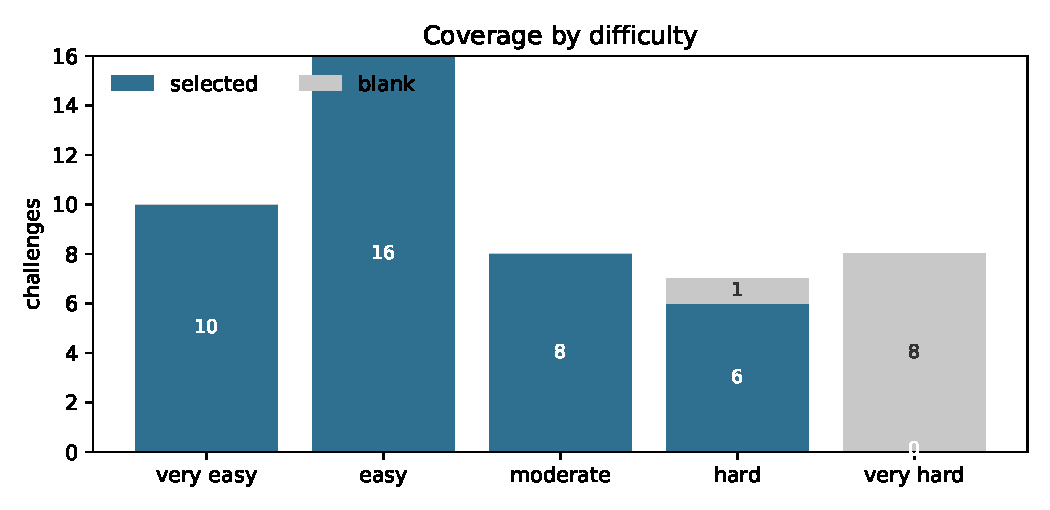
\includegraphics[width=0.48\linewidth]{figures/coverage_by_difficulty.pdf}
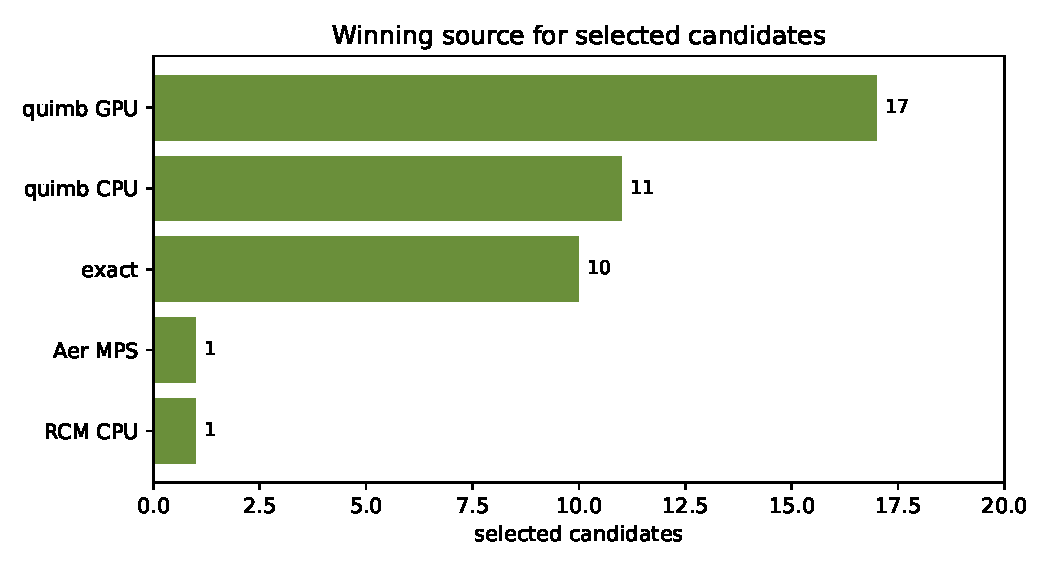
\includegraphics[width=0.48\linewidth]{figures/selected_source_counts.pdf}
\caption{Coverage and winning evidence sources. The nine missing rows are all hard or very hard.}
\end{figure}

\section*{What Was Tried}
\begin{longtable}{p{0.22\linewidth} p{0.51\linewidth} p{0.22\linewidth}}
\toprule
Method & Purpose and implementation & Outcome \\
\midrule
Exact statevector & Used Aer/statevector on small enough circuits to establish ground-truth peaks and bit ordering. & 10 exact answers. Used as calibration and highest-priority evidence. \\
Canonical graph/tree MPS & Ran Quimb tree-ordered MPS sampling on CPU and GPU, using sampled top bitstrings as candidate peaks. & Main source of approximate answers; strong on many easy/moderate rows and weak but usable on some hard rows. \\
Ordering fallbacks & Tried RCM, MST, degree, mid, fast, and identity orderings to change contraction behavior. & Added corroboration; RCM supplied the selected 56\_38 weak candidate. Long jobs were later cancelled. \\
Sparse computational-basis beam & Added a C++ top-K sparse branch propagator through RX/RZ/CX. & Rejected for answer selection: on known 16\_28 the exact answer was only rank 3. \\
Static QASM forensics & Counted gates, angle classes, pair repetitions, connectivity, leading one-qubit prefixes, and operation 5-gram similarity. & Confirmed all circuits are RX/RZ/CX/SWAP style, very-hard files are a distinct dense-obfuscation regime, and Clifford shortcuts are not appropriate. \\
Optimized-U3 transpilation & Transpiled the remaining blanks to U3+CX to reduce single-qubit gate count. & Reduced total gate count by roughly 39--42\% on blanks; not yet selected as evidence. \\
MPO unswapping & Patched the local Kremer-Dupuis style MPO cancellation/unswapping code: parameterized SABRE trials, fixed Quimb local expectation API, fixed quantum-op progress counting. & Calibrated on known 16\_28 in 93.26 s and recovered the exact answer. Unresolved runs were still active at report build time and are not counted as solved. \\
\bottomrule
\end{longtable}

\section*{Static Structure}
The QASM files use only \texttt{rx}, \texttt{rz}, \texttt{cx}, and sparse \texttt{swap} gates. Very-hard instances are
much larger and more internally similar to each other than to the easier sets. They also have dense leading single-qubit
prefixes and high all-to-all pair coverage. This drove the pivot toward structure-aware MPO cancellation rather than only
waiting for generic graph-MPS contractions.

\begin{figure}[H]
\centering
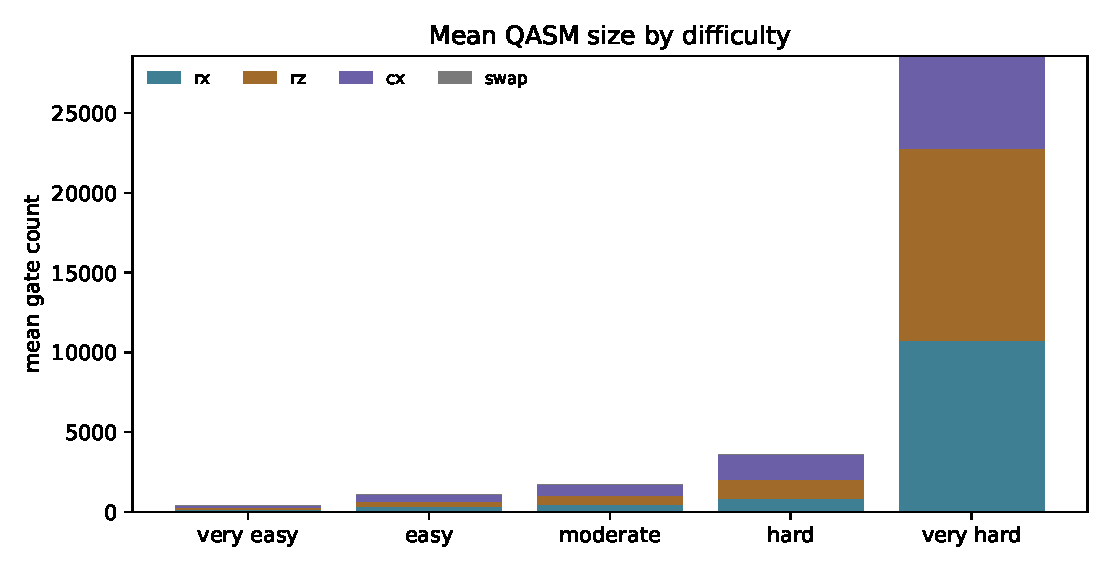
\includegraphics[width=0.48\linewidth]{figures/gate_counts_by_difficulty.pdf}
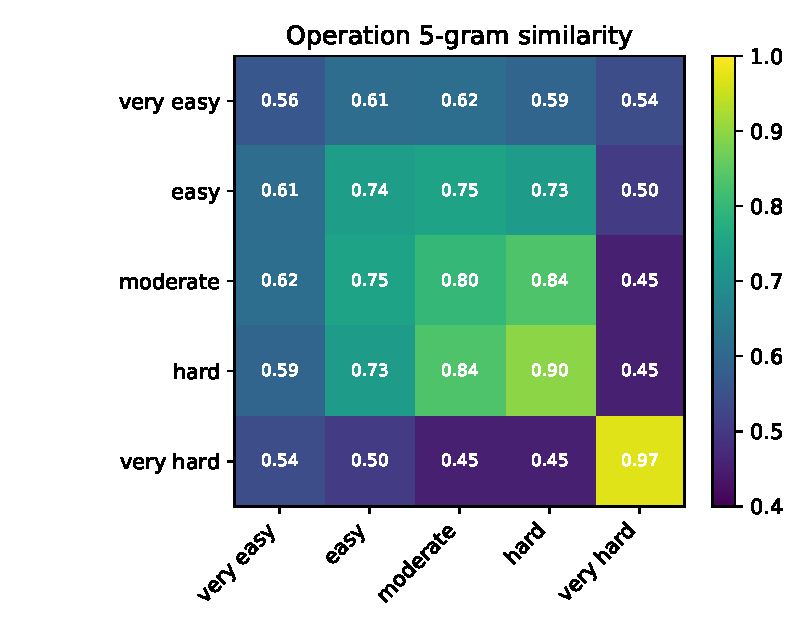
\includegraphics[width=0.42\linewidth]{figures/operation_similarity_heatmap.pdf}
\caption{Static QASM summary. Very-hard files are large and operation-sequence-similar to each other.}
\end{figure}

\section*{Exact Baseline}
The exact rows were used both as final answers and as calibration targets. The peak is visibly separated from the runner-up
on these cases, which made them useful for validating bit order and method behavior.

\begin{figure}[H]
\centering
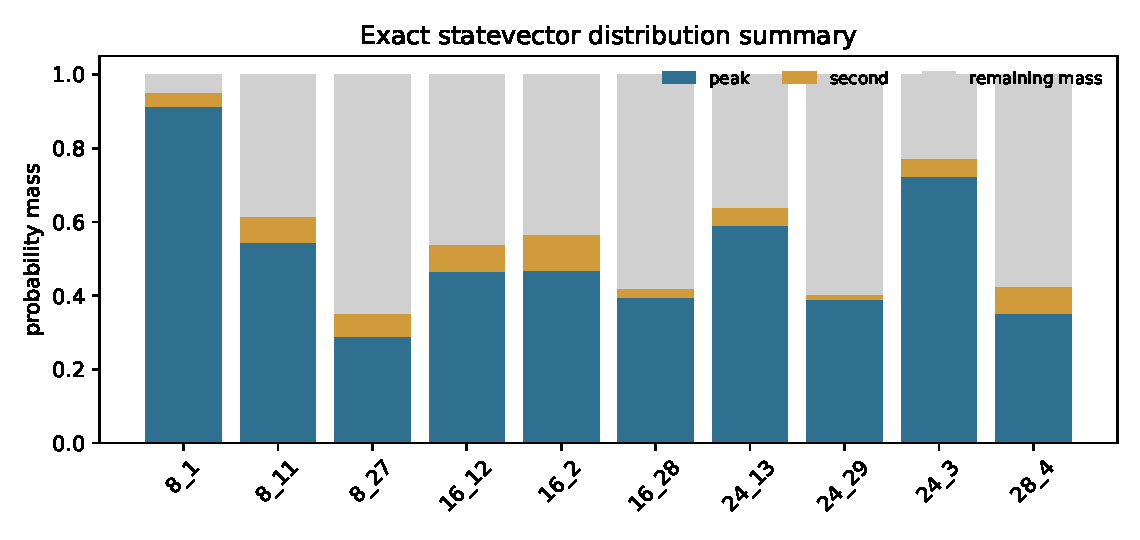
\includegraphics[width=0.78\linewidth]{figures/exact_peak_mass.pdf}
\caption{Exact statevector probability mass: peak, second-largest bitstring, and remaining mass.}
\end{figure}

\begin{longtable}{l r p{0.36\linewidth} r r r}
\toprule
Challenge & q & exact peak & peak prob. & second prob. & gap \\
\midrule
8\_1 & 8 & \texttt{\scriptsize 10101101} & 0.9126 & 0.0379 & 0.8747 \\
8\_11 & 8 & \texttt{\scriptsize 01001110} & 0.5454 & 0.0687 & 0.4768 \\
8\_27 & 8 & \texttt{\scriptsize 11001001} & 0.2879 & 0.0627 & 0.2252 \\
16\_12 & 16 & \texttt{\scriptsize 11110001\allowbreak 01101011} & 0.4665 & 0.0730 & 0.3936 \\
16\_2 & 16 & \texttt{\scriptsize 10101010\allowbreak 11001000} & 0.4670 & 0.0976 & 0.3694 \\
16\_28 & 16 & \texttt{\scriptsize 11010011\allowbreak 11011100} & 0.3962 & 0.0231 & 0.3731 \\
24\_13 & 24 & \texttt{\scriptsize 11111001\allowbreak 11110010\allowbreak 11010001} & 0.5912 & 0.0472 & 0.5441 \\
24\_29 & 24 & \texttt{\scriptsize 11010001\allowbreak 01111000\allowbreak 01001001} & 0.3901 & 0.0134 & 0.3767 \\
24\_3 & 24 & \texttt{\scriptsize 01111001\allowbreak 00001010\allowbreak 10001000} & 0.7240 & 0.0471 & 0.6769 \\
28\_4 & 28 & \texttt{\scriptsize 11111110\allowbreak 00101010\allowbreak 11011001\allowbreak 1111} & 0.3511 & 0.0735 & 0.2776 \\
\bottomrule
\end{longtable}

\section*{Approximate Tensor-Network Results}
For approximate rows, the sampled top fraction was the main confidence signal. Strong rows have a clear heavy bitstring.
Weak hard rows are retained because they are currently the best available candidates, but they should be interpreted as
low-confidence until corroborated.

\begin{figure}[H]
\centering
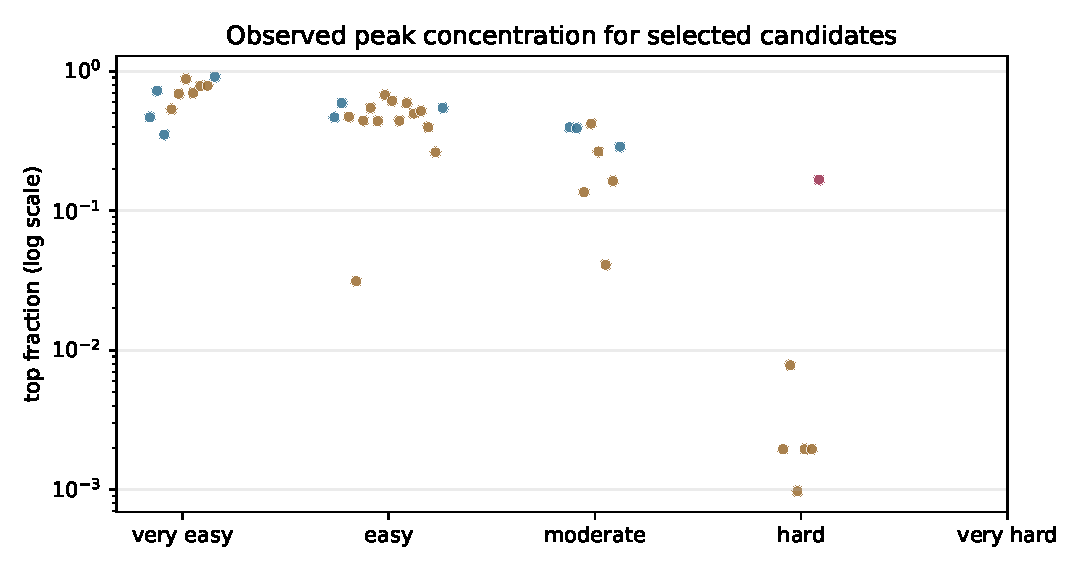
\includegraphics[width=0.48\linewidth]{figures/top_fraction_by_difficulty.pdf}
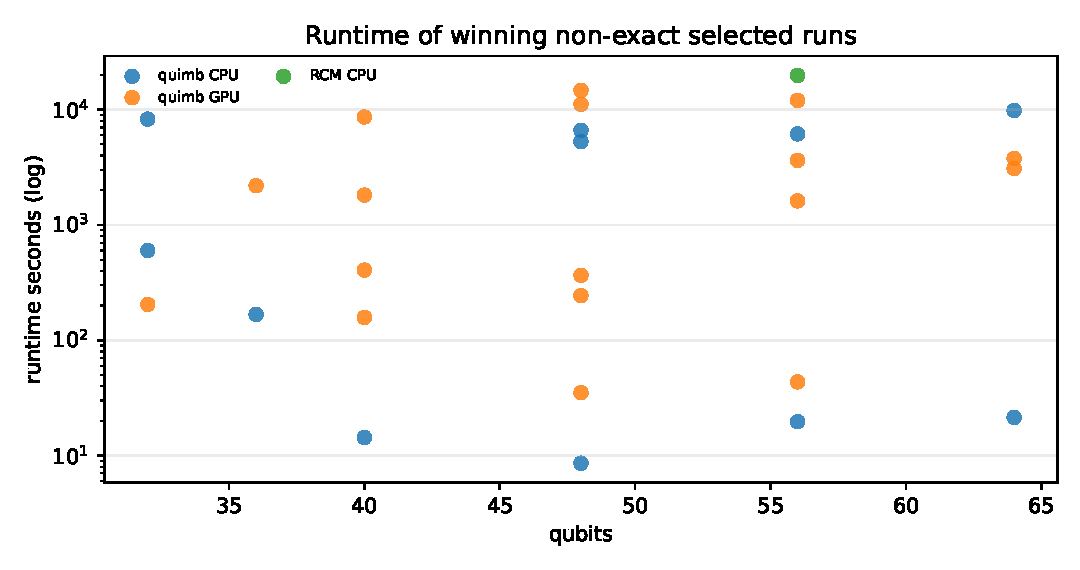
\includegraphics[width=0.48\linewidth]{figures/runtime_by_qubits.pdf}
\caption{Peak concentration and runtime for selected rows. The hard set contains several low-concentration candidates.}
\end{figure}

\begin{figure}[H]
\centering
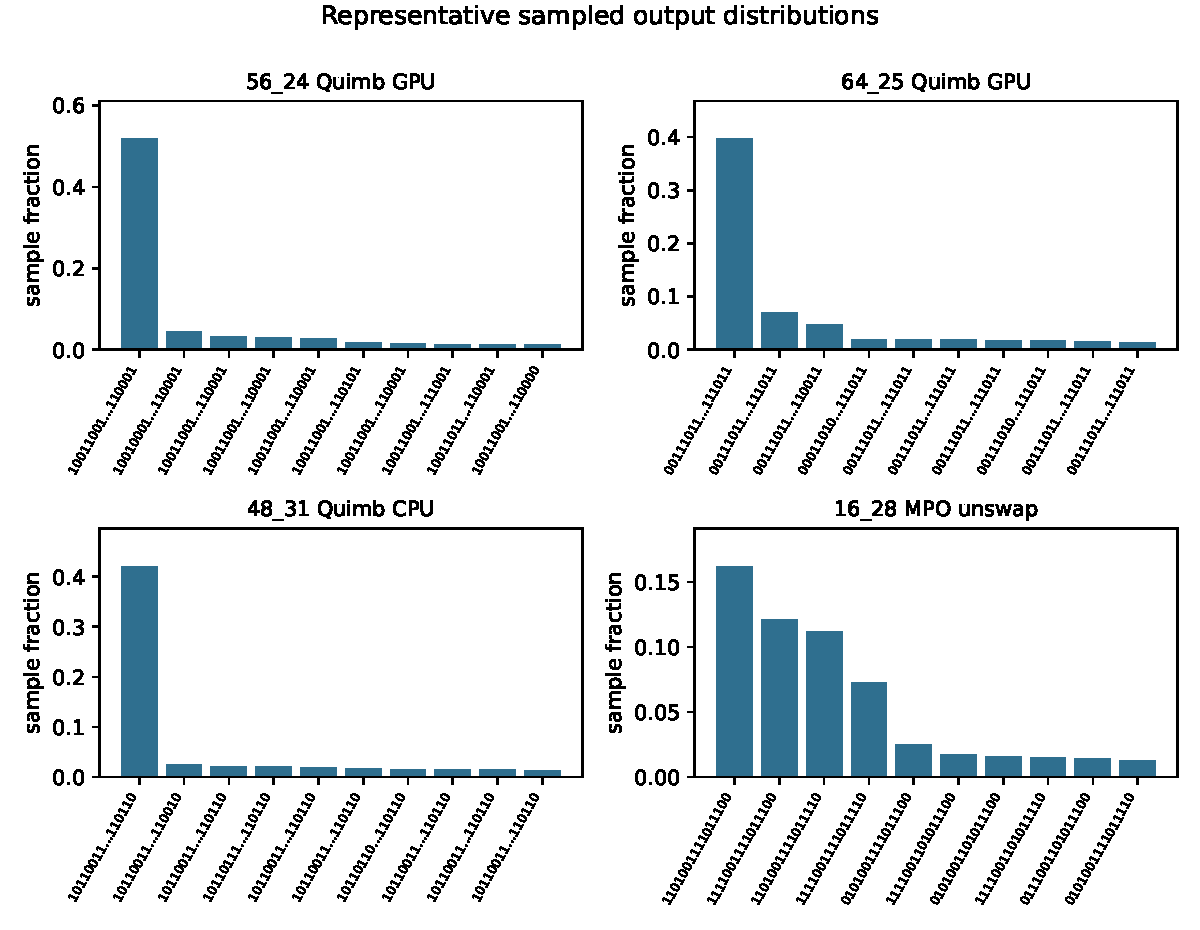
\includegraphics[width=0.86\linewidth]{figures/sample_distribution_examples.pdf}
\caption{Representative sampled distributions. The first three are selected Quimb candidates; the fourth is the MPO-unswap validation on 16\_28.}
\end{figure}

\subsection*{Weak Selected Rows}
\begin{longtable}{l l l r r p{0.35\linewidth}}
\toprule
Challenge & difficulty & source & top frac. & evidence & candidate \\
\midrule
40\_35 & hard & quimb GPU & 0.001953 & 3 & \texttt{\scriptsize 01011001\allowbreak 10101111\allowbreak 11100001\allowbreak 01010011\allowbreak 10001001} \\
48\_36 & hard & quimb GPU & 0.007812 & 3 & \texttt{\scriptsize 00111101\allowbreak 10110011\allowbreak 00110011\allowbreak 00100010\allowbreak 10011010\allowbreak 10111000} \\
48\_37 & hard & quimb GPU & 0.0009766 & 3 & \texttt{\scriptsize 10010100\allowbreak 10100011\allowbreak 01010100\allowbreak 10010100\allowbreak 10010001\allowbreak 01010001} \\
56\_38 & hard & RCM CPU & 0.001953 & 1 & \texttt{\scriptsize 10011001\allowbreak 01111000\allowbreak 00000100\allowbreak 11010101\allowbreak 10000100\allowbreak 10011101\allowbreak 10110001} \\
56\_39 & hard & quimb GPU & 0.001953 & 3 & \texttt{\scriptsize 10010111\allowbreak 00110101\allowbreak 01011111\allowbreak 11010110\allowbreak 11011011\allowbreak 00001010\allowbreak 01010000} \\
64\_41 & hard & Aer MPS & 0.167 & 1 & \texttt{\scriptsize 00010001\allowbreak 11010011\allowbreak 10011001\allowbreak 00111101\allowbreak 11000000\allowbreak 10001101\allowbreak 00011010\allowbreak 10110010} \\
32\_5 & very easy & quimb CPU & 0.5322 & 1 & \texttt{\scriptsize 00111000\allowbreak 10101010\allowbreak 00010000\allowbreak 00010000} \\
36\_6 & very easy & quimb CPU & 0.6885 & 1 & \texttt{\scriptsize 10011010\allowbreak 01111010\allowbreak 01001101\allowbreak 11001100\allowbreak 1000} \\
40\_7 & very easy & quimb CPU & 0.8789 & 1 & \texttt{\scriptsize 01101110\allowbreak 11010001\allowbreak 01001111\allowbreak 11100100\allowbreak 11000111} \\
48\_8 & very easy & quimb CPU & 0.6973 & 1 & \texttt{\scriptsize 00010010\allowbreak 01101110\allowbreak 01001111\allowbreak 11110010\allowbreak 10110011\allowbreak 10010100} \\
56\_9 & very easy & quimb CPU & 0.7812 & 1 & \texttt{\scriptsize 10010110\allowbreak 10110010\allowbreak 11101001\allowbreak 10010110\allowbreak 01110110\allowbreak 01100011\allowbreak 01010100} \\
64\_10 & very easy & quimb CPU & 0.7871 & 1 & \texttt{\scriptsize 00110100\allowbreak 10110001\allowbreak 11001011\allowbreak 10011001\allowbreak 00101100\allowbreak 01011111\allowbreak 01100101\allowbreak 00101011} \\
\bottomrule
\end{longtable}

\section*{Rejected or Not-Yet-Selected Paths}
The sparse beam search was attractive because it was fast, but its pruning bias failed calibration. In known 16\_28, the exact
answer was rank 3 rather than rank 1, so no sparse-beam guesses were promoted to selected answers. U3 optimization reduced
the remaining blank gate counts substantially, but its GPU pass was not completed before this report snapshot.

\begin{figure}[H]
\centering
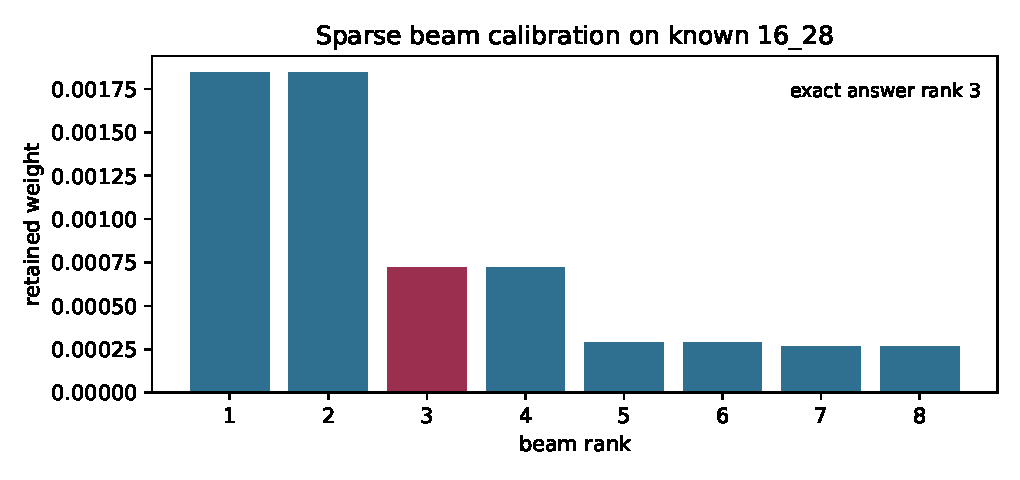
\includegraphics[width=0.45\linewidth]{figures/sparse_beam_calibration.pdf}
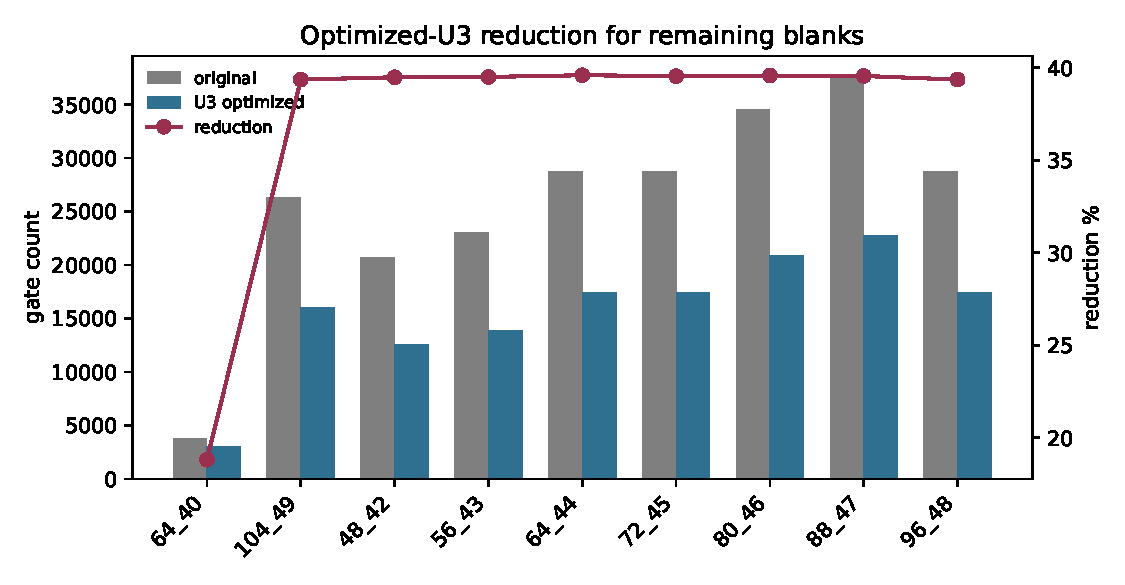
\includegraphics[width=0.53\linewidth]{figures/u3_reduction_remaining.pdf}
\caption{Left: sparse beam failed calibration. Right: U3 optimization reduced the remaining blank circuits but was not yet selected as evidence.}
\end{figure}

\begin{longtable}{l r r r r}
\toprule
Blank & q & original gates & U3 gates & reduction \\
\midrule
64\_40 & 64 & 3758 & 3051 & 18.8\% \\
104\_49 & 104 & 26361 & 15985 & 39.4\% \\
48\_42 & 48 & 20733 & 12547 & 39.5\% \\
56\_43 & 56 & 23004 & 13917 & 39.5\% \\
64\_44 & 64 & 28787 & 17389 & 39.6\% \\
72\_45 & 72 & 28777 & 17397 & 39.5\% \\
80\_46 & 80 & 34586 & 20898 & 39.6\% \\
88\_47 & 88 & 37660 & 22764 & 39.6\% \\
96\_48 & 96 & 28703 & 17406 & 39.4\% \\
\bottomrule
\end{longtable}

\section*{Current Slurm Snapshot}
The report is an as-of snapshot. Any active unresolved MPO-unswap jobs below were still running or pending when the PDF was built,
and their outputs are not counted in the \textbf{40/49} result.

\begin{longtable}{l l l r p{0.24\linewidth} p{0.24\linewidth}}
\toprule
JobID & state & elapsed & CPUs & name & node/reason \\
\midrule
34614255 & PENDING & 0:00 & 2 & peaked\_unswap\_rollup & (Dependency) \\
34614254\_[46-48\%5] & PENDING & 0:00 & 16 & peaked\_unswap\_unresolved & (JobArrayTaskLimit) \\
34614254\_45 & RUNNING & 3:12 & 16 & peaked\_unswap\_unresolved & erc-hpc-comp202 \\
34614254\_21 & RUNNING & 4:44 & 16 & peaked\_unswap\_unresolved & erc-hpc-comp192 \\
34614254\_41 & RUNNING & 4:44 & 16 & peaked\_unswap\_unresolved & erc-hpc-comp195 \\
34614254\_43 & RUNNING & 4:44 & 16 & peaked\_unswap\_unresolved & erc-hpc-vm064 \\
34614254\_44 & RUNNING & 4:44 & 16 & peaked\_unswap\_unresolved & erc-hpc-vm065 \\
\bottomrule
\end{longtable}

\section*{Method Summary}
\begin{longtable}{l r r r}
\toprule
Source & selected winners & candidate evidence rows & attempted evidence rows \\
\midrule
Aer MPS & 1 & 6 & 6 \\
exact & 10 & 10 & 10 \\
MPO unswap & 0 & 1 & 1 \\
quimb CPU & 11 & 36 & 36 \\
degree CPU & 0 & 1 & 1 \\
fast CPU & 0 & 5 & 5 \\
quimb GPU & 17 & 21 & 21 \\
RCM CPU & 1 & 16 & 16 \\
sparse beam & 0 & 5 & 5 \\
\bottomrule
\end{longtable}

\section*{Selected Candidate Table}
Full candidate bitstrings are shown in wrapped monospace chunks. Blank rows remain unsolved.

\scriptsize
\begin{longtable}{l l r p{0.36\linewidth} l l r r}
\toprule
Challenge & difficulty & q & candidate & source & validation & top frac. & evidence \\
\midrule
8\_1 & very easy & 8 & \texttt{\scriptsize 10101101} & exact & exact & 0.9126 & 2 \\
16\_2 & very easy & 16 & \texttt{\scriptsize 10101010\allowbreak 11001000} & exact & exact & 0.467 & 2 \\
24\_3 & very easy & 24 & \texttt{\scriptsize 01111001\allowbreak 00001010\allowbreak 10001000} & exact & exact & 0.724 & 2 \\
28\_4 & very easy & 28 & \texttt{\scriptsize 11111110\allowbreak 00101010\allowbreak 11011001\allowbreak 1111} & exact & exact & 0.3511 & 2 \\
32\_5 & very easy & 32 & \texttt{\scriptsize 00111000\allowbreak 10101010\allowbreak 00010000\allowbreak 00010000} & quimb CPU & unknown & 0.5322 & 1 \\
36\_6 & very easy & 36 & \texttt{\scriptsize 10011010\allowbreak 01111010\allowbreak 01001101\allowbreak 11001100\allowbreak 1000} & quimb CPU & unknown & 0.6885 & 1 \\
40\_7 & very easy & 40 & \texttt{\scriptsize 01101110\allowbreak 11010001\allowbreak 01001111\allowbreak 11100100\allowbreak 11000111} & quimb CPU & unknown & 0.8789 & 1 \\
48\_8 & very easy & 48 & \texttt{\scriptsize 00010010\allowbreak 01101110\allowbreak 01001111\allowbreak 11110010\allowbreak 10110011\allowbreak 10010100} & quimb CPU & unknown & 0.6973 & 1 \\
56\_9 & very easy & 56 & \texttt{\scriptsize 10010110\allowbreak 10110010\allowbreak 11101001\allowbreak 10010110\allowbreak 01110110\allowbreak 01100011\allowbreak 01010100} & quimb CPU & unknown & 0.7812 & 1 \\
64\_10 & very easy & 64 & \texttt{\scriptsize 00110100\allowbreak 10110001\allowbreak 11001011\allowbreak 10011001\allowbreak 00101100\allowbreak 01011111\allowbreak 01100101\allowbreak 00101011} & quimb CPU & unknown & 0.7871 & 1 \\
8\_11 & easy & 8 & \texttt{\scriptsize 01001110} & exact & exact & 0.5454 & 4 \\
16\_12 & easy & 16 & \texttt{\scriptsize 11110001\allowbreak 01101011} & exact & exact & 0.4665 & 4 \\
24\_13 & easy & 24 & \texttt{\scriptsize 11111001\allowbreak 11110010\allowbreak 11010001} & exact & exact & 0.5912 & 3 \\
32\_14 & easy & 32 & \texttt{\scriptsize 00000101\allowbreak 00110100\allowbreak 00010111\allowbreak 11101100} & quimb GPU & unknown & 0.4717 & 3 \\
36\_15 & easy & 36 & \texttt{\scriptsize 11011001\allowbreak 10111111\allowbreak 11011001\allowbreak 01111010\allowbreak 1111} & quimb GPU & unknown & 0.03125 & 3 \\
40\_16 & easy & 40 & \texttt{\scriptsize 01011101\allowbreak 01001110\allowbreak 01100011\allowbreak 10111001\allowbreak 10010110} & quimb GPU & unknown & 0.4424 & 4 \\
40\_17 & easy & 40 & \texttt{\scriptsize 00100101\allowbreak 01010111\allowbreak 00100100\allowbreak 00100010\allowbreak 00001001} & quimb GPU & unknown & 0.5459 & 4 \\
40\_18 & easy & 40 & \texttt{\scriptsize 01000001\allowbreak 10010010\allowbreak 00110111\allowbreak 10001111\allowbreak 11001110} & quimb GPU & unknown & 0.4395 & 3 \\
48\_19 & easy & 48 & \texttt{\scriptsize 01100101\allowbreak 01111011\allowbreak 00111110\allowbreak 00000101\allowbreak 11010011\allowbreak 10010000} & quimb GPU & unknown & 0.6738 & 2 \\
48\_20 & easy & 48 & \texttt{\scriptsize 10101010\allowbreak 01010010\allowbreak 10000110\allowbreak 10100000\allowbreak 10111100\allowbreak 10000000} & quimb GPU & unknown & 0.6123 & 3 \\
48\_21 & easy & 48 & \texttt{\scriptsize 11101010\allowbreak 11101010\allowbreak 11110101\allowbreak 00000110\allowbreak 10001000\allowbreak 00001001} & quimb GPU & unknown & 0.4414 & 3 \\
56\_22 & easy & 56 & \texttt{\scriptsize 11100100\allowbreak 10011001\allowbreak 00111100\allowbreak 10110110\allowbreak 01100000\allowbreak 01000101\allowbreak 11111011} & quimb GPU & unknown & 0.5898 & 2 \\
56\_23 & easy & 56 & \texttt{\scriptsize 01001101\allowbreak 00111111\allowbreak 11000001\allowbreak 01001110\allowbreak 11101110\allowbreak 00111111\allowbreak 00001101} & quimb GPU & unknown & 0.4971 & 2 \\
56\_24 & easy & 56 & \texttt{\scriptsize 10011001\allowbreak 00111110\allowbreak 11111110\allowbreak 11101011\allowbreak 10110101\allowbreak 00110010\allowbreak 11110001} & quimb GPU & unknown & 0.5176 & 4 \\
64\_25 & easy & 64 & \texttt{\scriptsize 00111011\allowbreak 11110000\allowbreak 11011011\allowbreak 11010110\allowbreak 00010000\allowbreak 01010011\allowbreak 01110000\allowbreak 01111011} & quimb GPU & unknown & 0.3965 & 4 \\
64\_26 & easy & 64 & \texttt{\scriptsize 01101010\allowbreak 10100011\allowbreak 01011101\allowbreak 10000111\allowbreak 00010110\allowbreak 11011001\allowbreak 11000110\allowbreak 01100110} & quimb GPU & unknown & 0.2617 & 3 \\
8\_27 & moderate & 8 & \texttt{\scriptsize 11001001} & exact & exact & 0.2879 & 2 \\
16\_28 & moderate & 16 & \texttt{\scriptsize 11010011\allowbreak 11011100} & exact & exact & 0.3962 & 6 \\
24\_29 & moderate & 24 & \texttt{\scriptsize 11010001\allowbreak 01111000\allowbreak 01001001} & exact & exact & 0.3901 & 4 \\
32\_30 & moderate & 32 & \texttt{\scriptsize 10011000\allowbreak 01001111\allowbreak 01111011\allowbreak 11010111} & quimb CPU & unknown & 0.1357 & 2 \\
48\_31 & moderate & 48 & \texttt{\scriptsize 10110011\allowbreak 10001010\allowbreak 11111111\allowbreak 10101011\allowbreak 10110110\allowbreak 00110110} & quimb CPU & unknown & 0.4209 & 2 \\
48\_32 & moderate & 48 & \texttt{\scriptsize 01110101\allowbreak 01110111\allowbreak 10001110\allowbreak 01010101\allowbreak 01011011\allowbreak 10001110} & quimb CPU & unknown & 0.2656 & 2 \\
56\_33 & moderate & 56 & \texttt{\scriptsize 11001001\allowbreak 10010100\allowbreak 11110101\allowbreak 00100010\allowbreak 01010111\allowbreak 11110111\allowbreak 01010000} & quimb CPU & unknown & 0.04102 & 2 \\
64\_34 & moderate & 64 & \texttt{\scriptsize 00110101\allowbreak 00010011\allowbreak 00111010\allowbreak 11101001\allowbreak 01001011\allowbreak 00101101\allowbreak 10011110\allowbreak 11100110} & quimb CPU & unknown & 0.1631 & 2 \\
40\_35 & hard & 40 & \texttt{\scriptsize 01011001\allowbreak 10101111\allowbreak 11100001\allowbreak 01010011\allowbreak 10001001} & quimb GPU & unknown & 0.001953 & 3 \\
48\_36 & hard & 48 & \texttt{\scriptsize 00111101\allowbreak 10110011\allowbreak 00110011\allowbreak 00100010\allowbreak 10011010\allowbreak 10111000} & quimb GPU & unknown & 0.007812 & 3 \\
48\_37 & hard & 48 & \texttt{\scriptsize 10010100\allowbreak 10100011\allowbreak 01010100\allowbreak 10010100\allowbreak 10010001\allowbreak 01010001} & quimb GPU & unknown & 0.0009766 & 3 \\
56\_38 & hard & 56 & \texttt{\scriptsize 10011001\allowbreak 01111000\allowbreak 00000100\allowbreak 11010101\allowbreak 10000100\allowbreak 10011101\allowbreak 10110001} & RCM CPU & unknown & 0.001953 & 1 \\
56\_39 & hard & 56 & \texttt{\scriptsize 10010111\allowbreak 00110101\allowbreak 01011111\allowbreak 11010110\allowbreak 11011011\allowbreak 00001010\allowbreak 01010000} & quimb GPU & unknown & 0.001953 & 3 \\
64\_40 & hard & 64 &  &  &  &  & 0 \\
64\_41 & hard & 64 & \texttt{\scriptsize 00010001\allowbreak 11010011\allowbreak 10011001\allowbreak 00111101\allowbreak 11000000\allowbreak 10001101\allowbreak 00011010\allowbreak 10110010} & Aer MPS & unstable\_top1\_vs\_aggregate & 0.167 & 1 \\
48\_42 & very hard & 48 &  &  &  &  & 0 \\
56\_43 & very hard & 56 &  &  &  &  & 0 \\
64\_44 & very hard & 64 &  &  &  &  & 0 \\
72\_45 & very hard & 72 &  &  &  &  & 0 \\
80\_46 & very hard & 80 &  &  &  &  & 0 \\
88\_47 & very hard & 88 &  &  &  &  & 0 \\
96\_48 & very hard & 96 &  &  &  &  & 0 \\
104\_49 & very hard & 104 &  &  &  &  & 0 \\
\bottomrule
\end{longtable}
\normalsize

\section*{Conclusions}
The practical output of the session is a 40-row candidate answer set and a clear split between reliable and weak evidence.
The exact and high-top-fraction Quimb rows are the most defensible. The hard weak rows should be treated as provisional.
The best next direction is not another unconstrained graph-MPS sweep: it is bounded MPO-unswapping or optimized-U3 GPU runs
with calibration checks and immediate collector refreshes.

\end{document}
